\section{Règles de changement d'états et moteur de jeu}

\subsection{Règles}
Outre l'initialisation du jeu et la fin du jeu dont nous ne parlerons pas pour l'instant, on peut décomposer notre jeu en 2 états principaux: la carte, et l'intérieur des salles. Le jeu se termine lorsque toutes les salles sont parcourues sans mort des joueurs, ou lorsque que les joueurs sont morts.

\subsubsection{La carte}
A partir de la carte, seule une action est possible : passer à la salle suivante. Il n'y a pour l'instant qu'un unique chemin possible. Une fois que la salle suivante est sélectionnée, on rentre à l'intérieur de cette salle.

\subsubsection{L'intérieur des salles}
\textbf{Salle d'ennemis}

En entrant dans une salle d'ennemis, les joueurs affrontent 1 ou plusieurs ennemis. Les tours se déroulent selon la logique suivante: le joueur 1 joue son tour, puis le joueur 2 s'il existe, puis l'ennemi 1, l'ennemi 2 et 3 s'ils existent. Au début de son tour, un joueur voit son énergie réinitialisée à 3, ses buffs et débuffs baissent de 1, et il pioche 5 nouvelles cartes de sa pile de pioche ( s'il n'y a plus assez de cartes dans la pioche, la défausse est mélangée et forme la nouvelle pioche) vers sa main. Les seules actions disponibles sont passer le tour ou jouer une carte. 
\par Tant que le joueur possède l'énergie suffisante, il peut joueur des cartes. Pour jouer une carte, il sélectionne la carte en cliquant dessus, puis séléctionne la cible en cliquant dessus. S'il tente de jouer une carte avec un coût supérieur à son énergie, ou s'il sélectionne une mauvaise cible pour cette carte, elle ne sera pas jouée et restera dans sa main. Lorsqu'une carte est jouée, l'énergie du joueur baisse d'autant que le coût de la carte, ses effets sont appliqués (attaque, block, ajout de bonus ou malus, pioche, défausse, soin...), puis elle est défaussée. La taille maximale de la main est 7.
\par Lorsque le joueur décide de finir son tour (en appuyant sur "end turn"), toutes les cartes qu'il avait dans sa main sont mises dans la pile de défausse. L'entité suivante joue son tour.
\par Si c'est le tour d'un ennemi, l'ennemi réalise son action (attaque, block, application d'un bonus/malus...) sur une cible valide.
\par Une fois que tous les ennemis sont morts (soit que leur vie est à 0), les joueurs peuvent sélectionner une carte de récompense. Le dernier ennemi tué défini les cartes obtenues en récompense. Une seule carte peut être sélectionnée par personne, mais cette carte peut être la même pour les deux joueurs. La carte sélectionnée est ajoutée au deck du joueur. Le deck possède déjà 15 cartes, alors le joueur doit définitivement enlever une carte de son deck avant de pouvoir ajouter la nouvelle. Les joueurs peuvent également choisir de ne pas sélectionner de carte. Après cette phase, les joueurs sortent de la salle et peuvent sélectionner la suivante depuis la carte.

\textbf{Salle d'entraînement}

En entrant dans une salle d'entraînement, trois cartes sont proposées. Les joueurs peuvent choisir une de ces cartes et l'ajouter à son deck (si le deck fait déjà 15 cartes, une carte doit préalablement être retirée). Cette carte peut être la même pour les deux joueurs. Ils peuvent aussi choisir de passer directement à la salle suivante en appuyant sur "pass". Ils passent alors à la salle suivante.

\textbf{Salle de repos}

En entrant dans une salle de repos, les joueurs ont deux choix possibles : se reposer et se soigner d'un nombre de PV indiqué, ou méditer et gagner un gain définitif en valeur d'attaque et de block. 

\clearpage
\subsection{Conception logiciel}

Les figures qui suivent présentent notre diagramme de classe sous forme de diagramme UML.

\begin{figure}[hp]
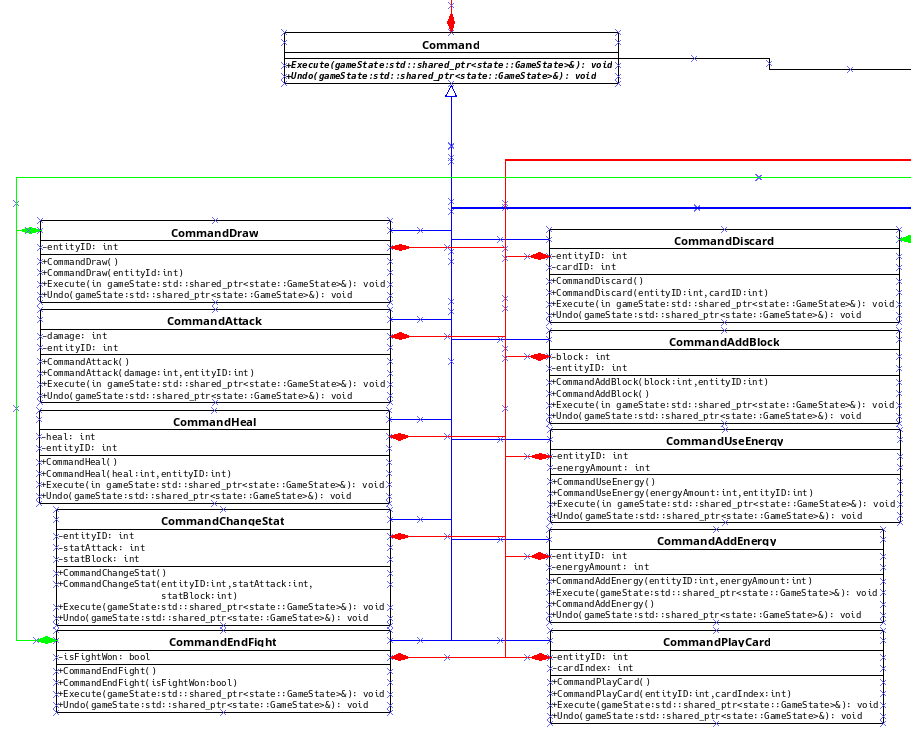
\includegraphics[width=0.6\paperheight]{images/engine1.png}
\caption{\label{uml:engine}Quelques commandes.} 
\end{figure}

\begin{figure}[hp]
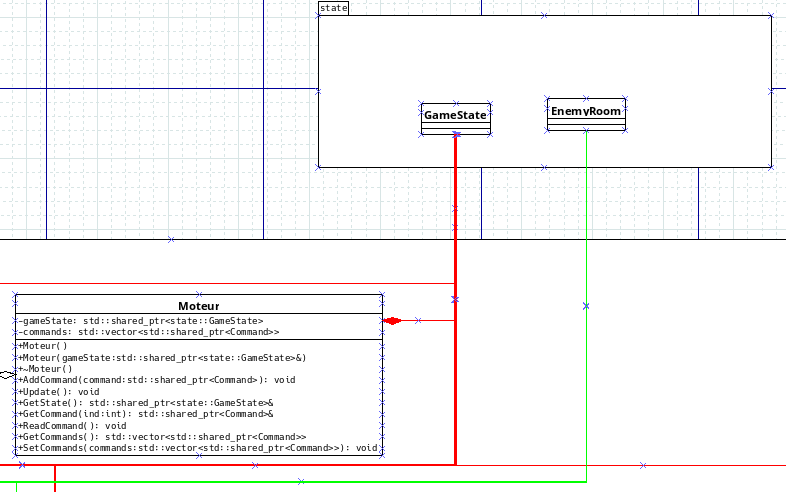
\includegraphics[width=0.5\paperheight]{images/engine2.png}
\caption{\label{uml:engine}Diagramme des classes de moteur de jeu.} 
\end{figure}

\begin{landscape}
\begin{figure}[hp]
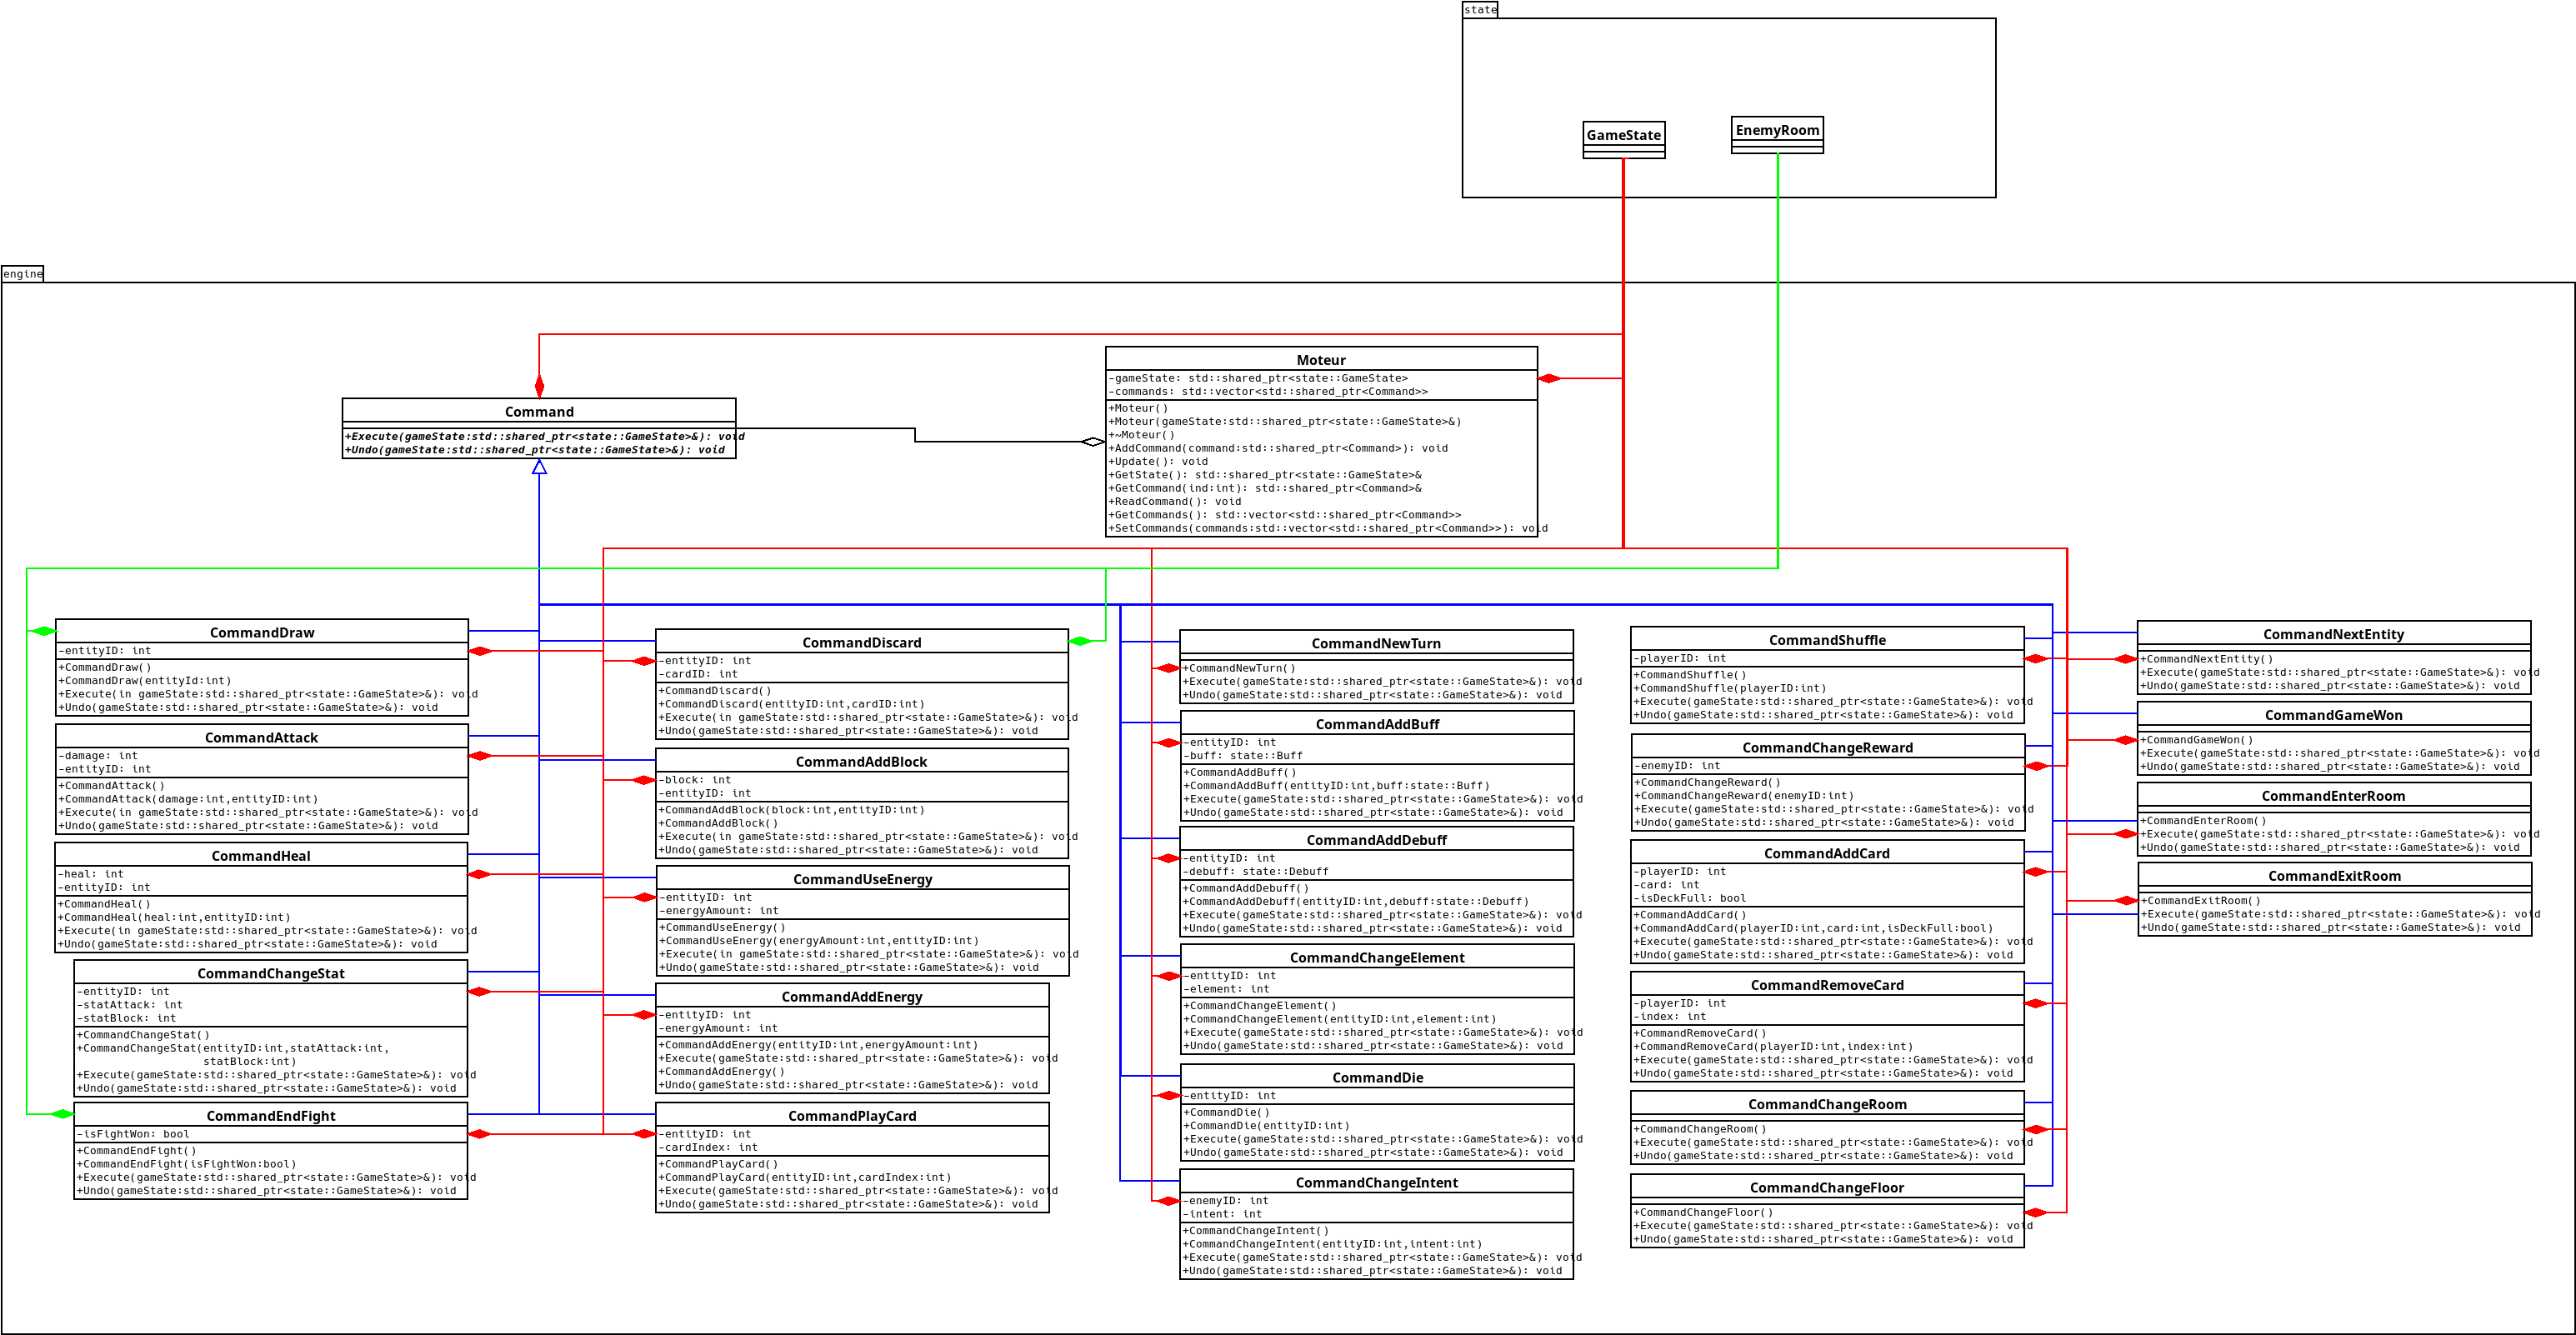
\includegraphics[width=0.9\paperheight]{images/engine.png}
\caption{\label{uml:engine}Diagramme des classes de moteur de jeu.} 
\end{figure}
\end{landscape}

\newpage
